%%%%%%%%%%%%%%%%%%%%%%%%%%%%%%%%%%%%%%%%%%%%%%%%%%%%%%%%%%%%%%%%%%%%%%%%%%%%%%%%%%%%%%%%%%%%%%%%
%
% CS484 Written Question Template
%
% Acknowledgements:
% The original code is written by Prof. James Tompkin (james_tompkin@brown.edu).
% The second version is revised by Prof. Min H. Kim (minhkim@kaist.ac.kr).
%
% This is a LaTeX document. LaTeX is a markup language for producing 
% documents. Your task is to fill out this document, then to compile 
% it into a PDF document. 
%
% 
% TO COMPILE:
% > pdflatex thisfile.tex
%
% If you do not have LaTeX and need a LaTeX distribution:
% - Personal laptops (all common OS): www.latex-project.org/get/
% - We recommend latex compiler miktex (https://miktex.org/) for windows,
%   macTex (http://www.tug.org/mactex/) for macOS users.
%   And TeXstudio(http://www.texstudio.org/) for latex editor.
%   You should install both compiler and editor for editing latex.
%   The another option is Overleaf (https://www.overleaf.com/) which is 
%   an online latex editor.
%
% If you need help with LaTeX, please come to office hours. 
% Or, there is plenty of help online:
% https://en.wikibooks.org/wiki/LaTeX
%
% Good luck!
% Min and the CS484 staff
%
%%%%%%%%%%%%%%%%%%%%%%%%%%%%%%%%%%%%%%%%%%%%%%%%%%%%%%%%%%%%%%%%%%%%%%%%%%%%%%%%%%%%%%%%%%%%%%%%
%
% How to include two graphics on the same line:
% 
% \includegraphics[width=0.49\linewidth]{yourgraphic1.png}
% \includegraphics[width=0.49\linewidth]{yourgraphic2.png}
%
% How to include equations:
%
% \begin{equation}
% y = mx+c
% \end{equation}
% 
%%%%%%%%%%%%%%%%%%%%%%%%%%%%%%%%%%%%%%%%%%%%%%%%%%%%%%%%%%%%%%%%%%%%%%%%%%%%%%%%%%%%%%%%%%%%%%%%

\documentclass[11pt]{article}

\usepackage[english]{babel}
\usepackage[utf8]{inputenc}
\usepackage[colorlinks = true,
            linkcolor = blue,
            urlcolor  = blue]{hyperref}
\usepackage[a4paper,margin=1.5in]{geometry}
\usepackage{stackengine,graphicx}
\usepackage{fancyhdr}
\setlength{\headheight}{15pt}
\usepackage{microtype}
\usepackage{times}

% From https://ctan.org/pkg/matlab-prettifier
\usepackage[numbered,framed]{matlab-prettifier}

\frenchspacing
\setlength{\parindent}{0cm} % Default is 15pt.
\setlength{\parskip}{0.3cm plus1mm minus1mm}

\pagestyle{fancy}
\fancyhf{}
\lhead{Homework 4 Questions}
\rhead{CS 484}
\rfoot{\thepage}

\date{}

\title{\vspace{-1cm}Homework 4 Questions}


\begin{document}
\maketitle
\vspace{-3cm}
\thispagestyle{fancy}

\section*{Instructions}
\begin{itemize}
  \item 4 questions.
  \item Write code where appropriate.
  \item Feel free to include images or equations.
  \item Please make this document anonymous.
  \item \textbf{Please use only the space provided and keep the page breaks.} Please do not make new pages, nor remove pages. The document is a template to help grading.
  \item If you really need extra space, please use new pages at the end of the document and refer us to it in your answers.
\end{itemize}

\section*{Questions}

\paragraph{Q1:} Imagine we were tasked with designing a feature point which could match all of the following three pairs of images. Which real world phenomena and camera effects might cause us problems?
Use the MATLAB function \href{https://www.mathworks.com/help/images/ref/corner.html}{$corner$} to investigate. $corner(I,1000)$.

\emph{RISHLibrary} | \emph{Chase} | \emph{LaddObservatory}

%%%%%%%%%%%%%%%%%%%%%%%%%%%%%%%%%%%
\paragraph{A1:} As using q1.m attached inside this folder, I could find the corners as like pictures attached like below.

\begin{figure}[h]
    \centering
    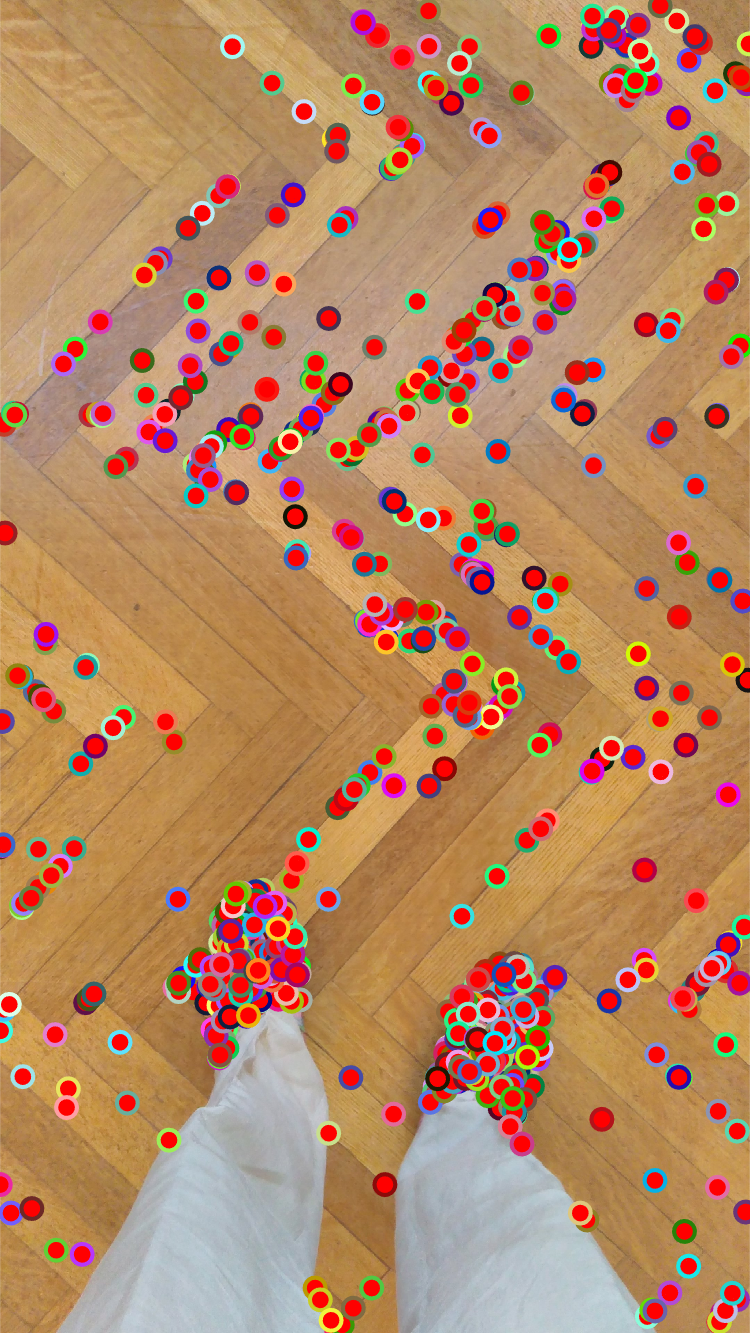
\includegraphics[width=1cm]{RL1.png}
    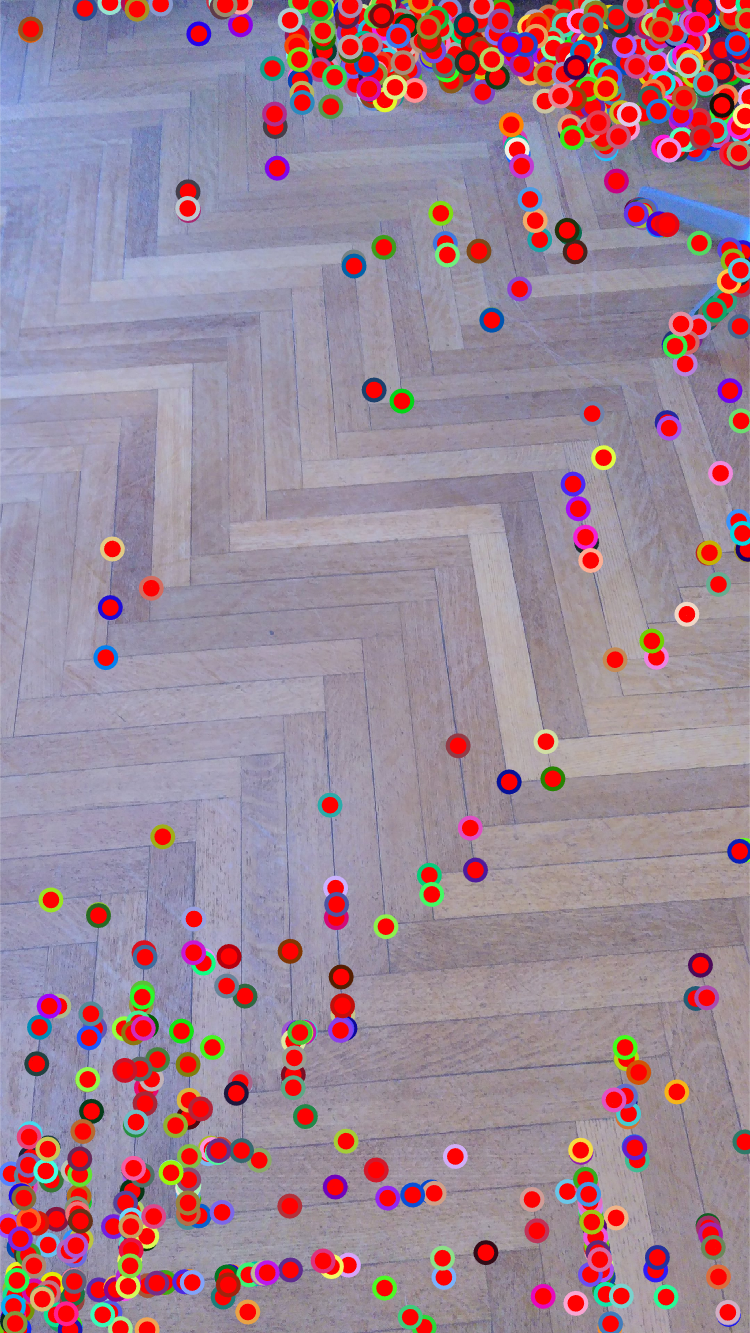
\includegraphics[width=1cm]{RL2.png}
    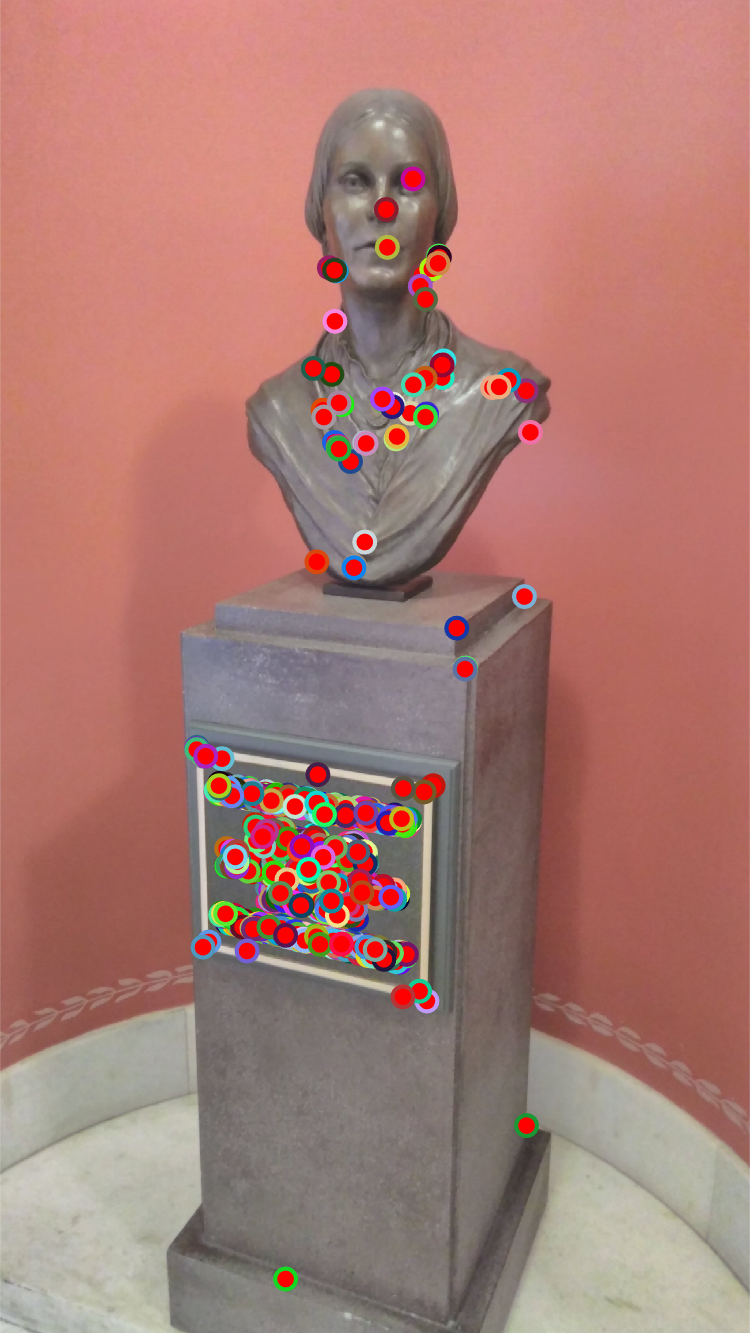
\includegraphics[width=1cm]{C1.png}
    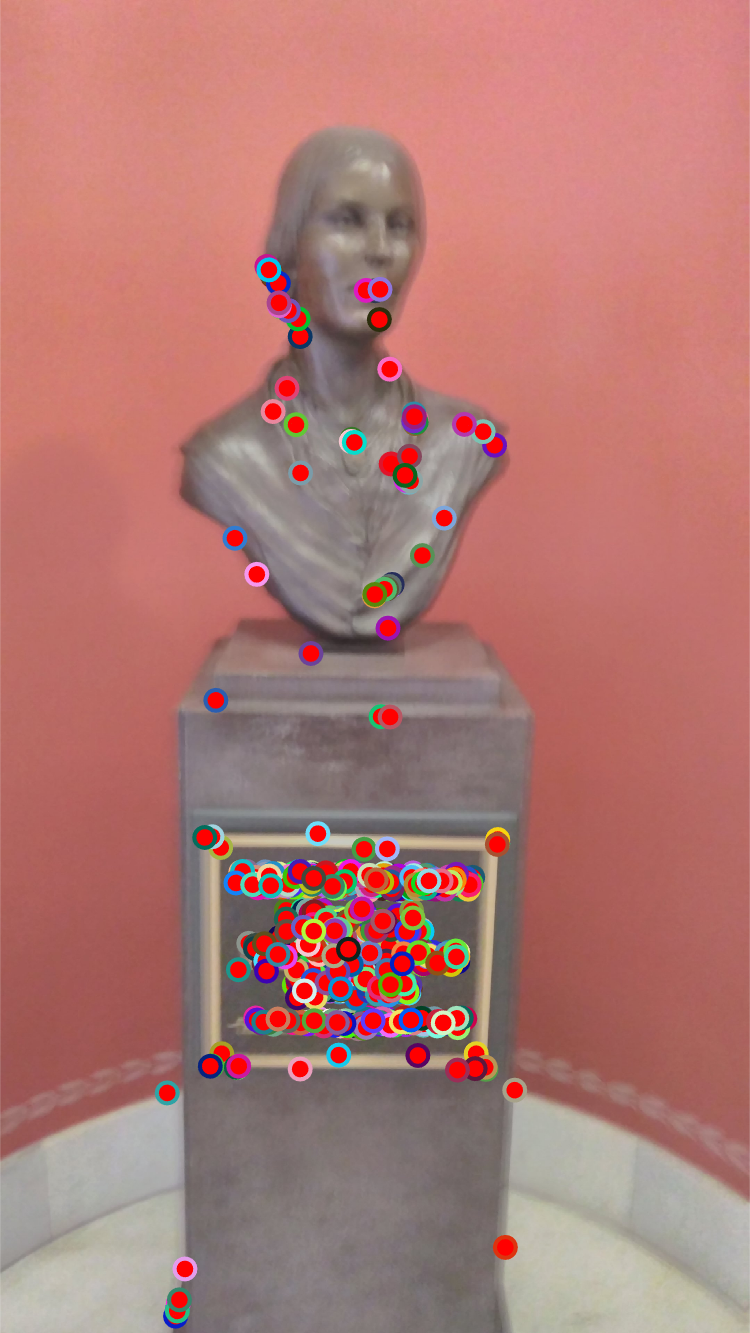
\includegraphics[width=1cm]{C2.png}
    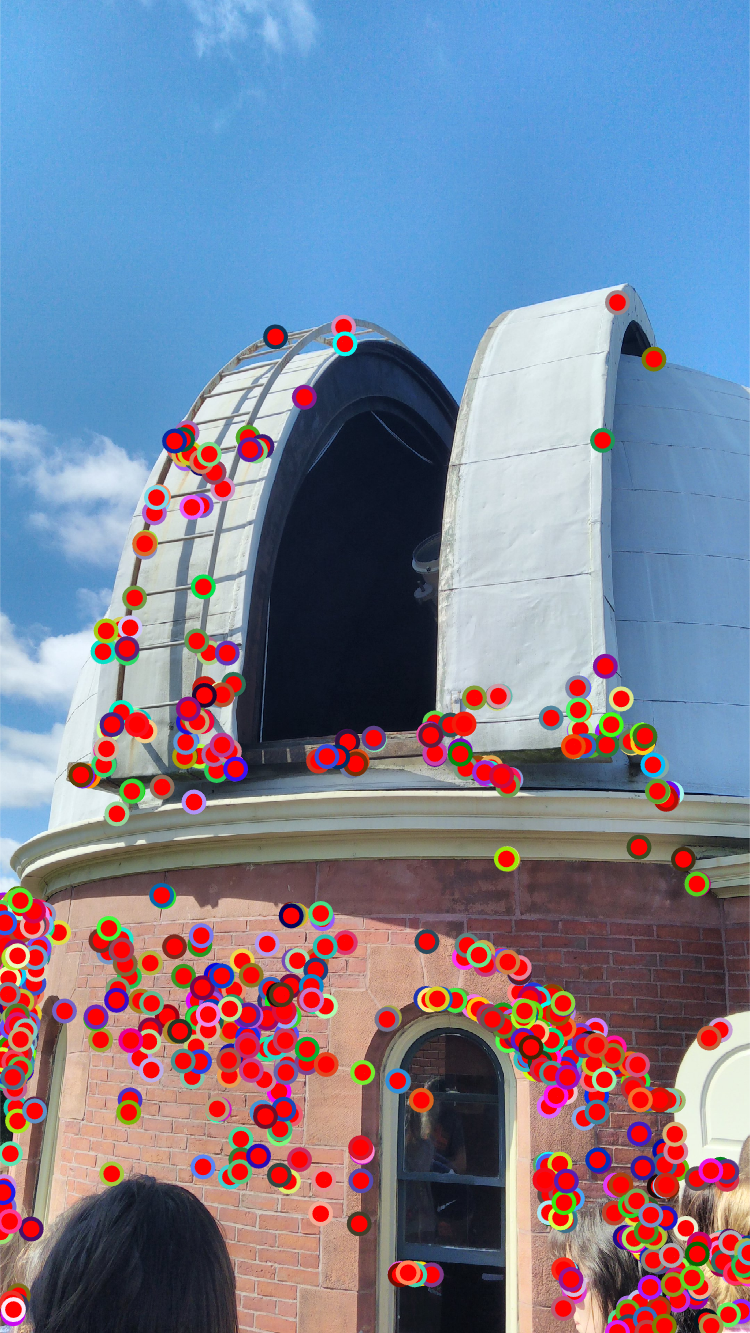
\includegraphics[width=1cm]{LO1.png}
    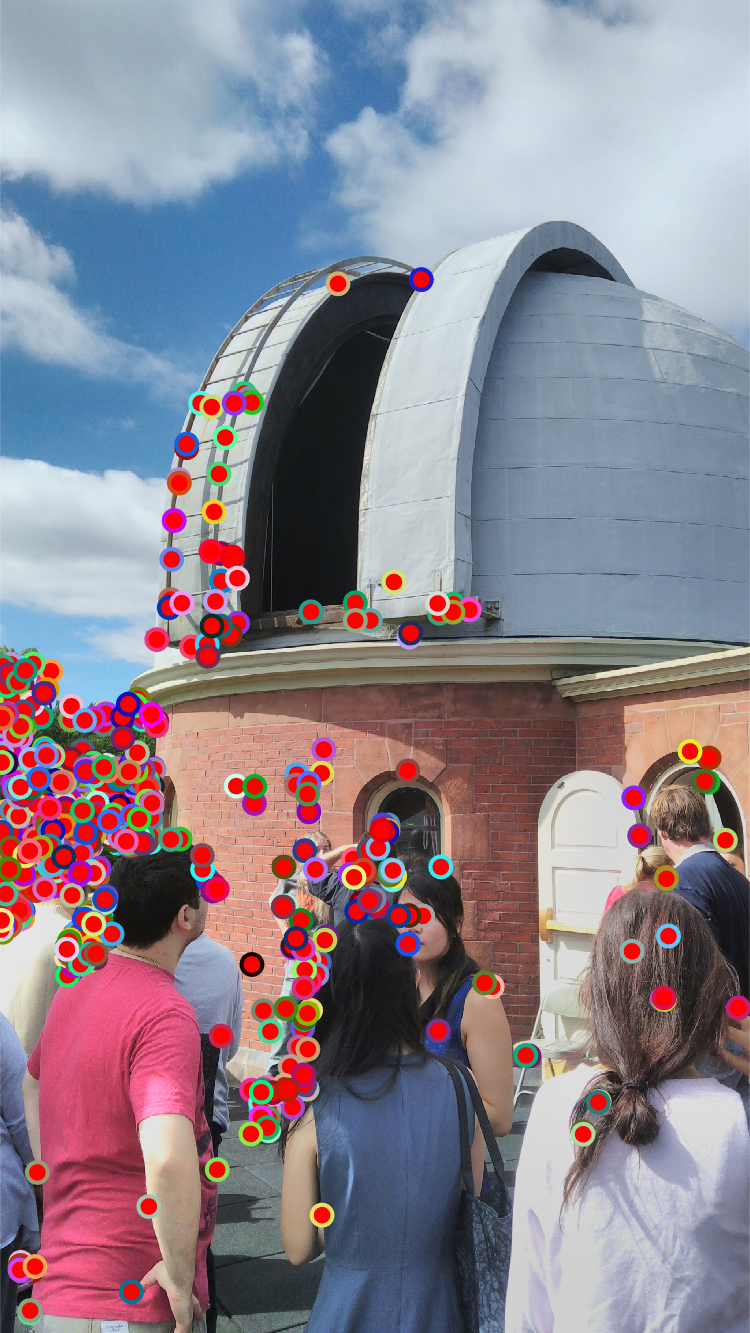
\includegraphics[width=1cm]{LO2.png}
    \caption{\emph{Left:} RISH Library \emph{Center:} Chase \emph{Right:} Ladd Observatory}
    \label{fig:result1}
\end{figure}

As we can easily find out from the pictures given above, if a new object appears, the feature points could vary severely. Also if the camera angle changes in a big difference, the corners could be detected with each of points have a big gap between itself. Specular highlighting problem also can be seen.

%%%%%%%%%%%%%%%%%%%%%%%%%%%%%%%%%%%

% Please leave the pagebreak
\pagebreak
\paragraph{Q2:} In designing our feature point, what characteristics might we wish it to have? Describe the fundamental trade-off between feature point invariance and discriminative power. How should we design for this trade-off?

%%%%%%%%%%%%%%%%%%%%%%%%%%%%%%%%%%%
\paragraph{A2:} Each feature point should be different from other feature point by having its own characteristical value in order to differ itself with another. But, in the same time, it should be detected as an identical point if we have another picture of the object taken in a different point of view, which it needs to be a particular point regardless of its direction. It also should ignore sudden change of colors or brightness, but the shape should be crucial to check if two or more feature points are identical or not.

To implement it, we'd love to calculate the gradient value of the blurred image using Gaussian filter which takes values disregards to the color of the picture. To identify the gradient value, making a cell grid around the feature point and divide the unique value made up from gradients from which from the value of feature point itself. It would wipe out the factor of the direction aligned by the grid.



%%%%%%%%%%%%%%%%%%%%%%%%%%%%%%%%%%%

% Please leave the pagebreak
\pagebreak
\paragraph{Q3:} In the Harris corner detector, what do the eigenvalues of the `M' second moment matrix represent? Discuss both how they relate to image intensity and how we can interpret them geometrically.

%%%%%%%%%%%%%%%%%%%%%%%%%%%%%%%%%%%
\paragraph{A3:} The eigenvalues of the second moment matrix represent the gradient values - both the intensity and direction for each pixels within the cell. To relate with image intensity, we would like to calculate the Harris value, to make an unique value to recognize the point only with identical factors. Interpreting it geometrically, we will divide the directions into 8~36 directions and stick it to the nearest direction. By such, we can easily identify direction and intensity for the total intensity for all pixels within the cell.



%%%%%%%%%%%%%%%%%%%%%%%%%%%%%%%%%%%


% Please leave the pagebreak
\pagebreak
\paragraph{Q4:} Explain the difference between the Euclidean distance and the cosine similarity metrics between descriptors. What might their geometric interpretations reveal about when each should be used? Given a distance metric, what is a good method for feature descriptor matching and why?

%%%%%%%%%%%%%%%%%%%%%%%%%%%%%%%%%%%
\paragraph{A4:} Euclidean distance is the linear distance between two points in a 2D-based Euclidean coordinate. Cosine similarity is the angular distance between two point vectors in a 2D-based polar coordinate. Euclidean distance should be used because it can easily check the linear distance between points, which is what we want to use as recognizing factors to easily find out if two points are close enough or not. For given Euclidean distance, we can compare the values of the most nearest point and second nearest point and get the ratio of it. It would check if the match of points are certain or not.



%%%%%%%%%%%%%%%%%%%%%%%%%%%%%%%%%%%


% If you really need extra space, uncomment here and use extra pages after the last question.
% Please refer here in your original answer. Thanks!
%\pagebreak
%\paragraph{AX.X Continued:} Your answer continued here.



\end{document}
